\chapter{An Overview of the Genome Properties Database, InterPro, and 
InterProScan5} \label{genome-properties} 

The architecture and implementation of Micromeda's components, such as Pygenprop 
and Micromeda-Client, are tied closely to the structure of the Genome Properties 
database. Thus, it is pertinent to discuss the database's structure. As 
mentioned in Section \ref{micromeda-overview}, Micromeda uses Pygenprop to 
predict the biochemical pathways possessed by an organism. These predictions are 
made by providing Pygenprop with a copy of the Genome Properties database and 
the output of running InterProScan5 on the organism's predicted proteins. In 
addition to discussing the structure of the Genome Properties database, this 
chapter will also discuss how domain annotations produced by InterProScan5 are 
combined with mappings from the Genome Properties database to generate pathway 
predictions.

\section{Protein Domains and Their Use as Markers of Enzyme Function}

A protein domain is a conserved subset of a protein's sequence that carries out 
a specific function and is evolutionarily conserved \cite{ren2008conservation}. 
These domains are associated with distinct sequence motifs, which are patterns 
in the protein's amino acid sequence \cite{ren2008conservation}. All enzymes 
have an active site 
(\href{http://en.wikipedia.org/wiki/Active_site}{en.wikipedia.org/wiki/Active\_site}), 
and this active site often has a unique sequence motif. This motif can be used 
to identify specific enzymes or enzyme families uniquely 
\cite{ren2008conservation}. 

The Genome Properties database takes advantage of this identifiability to map 
from combinations of protein domains to enzymes that carry out pathway steps. 
\cite{richardson2018genome}. This mapping is in contrast to most other pathway 
databases, which map from whole proteins to biochemical pathways. If all the 
required domains for a pathway step are present in an organism's proteins, then 
the step is considered present. The domains used as markers by the Genome 
Properties database are those catalogued within the InterPro consortium of 
protein databases \cite{apweiler2000interpro,richardson2018genome}. 

\section{The InterPro Consortium of Protein Databases} \label{InterProDatabases}

Because the enzymes that carry out elements of metabolism in different organisms 
are highly similar and often evolutionarily related, it is useful to categorize 
proteins into groups that carry out a single function or share specific domains. 
Protein databases record the function of these groups of proteins and their 
domains and also store copies of their sequences. The InterPro consortium 
\cite{apweiler2000interpro,hunter2008interpro,Hunter2009} contains fourteen 
child databases \cite{finn2016interpro,Hunter2009} (Fig. 
\ref{fig:interpro-databases}). In addition to the member databases, the 
consortium also provides the InterPro database 
\cite{hunter2008interpro,finn2016interpro}, which is a meta-database that allows 
for mapping between identical records for the same protein or domain groups 
across member databases. Each protein or domain catalogued is given a global 
InterPro identifier (\textit{e}.\textit{g}., IPRXXXX) that is mapped to multiple identifiers for 
the same protein or domain within member databases (\textit{e}.\textit{g}., PFXXXX or TFXXXX) 
\cite{hunter2008interpro,finn2016interpro}.

An import feature of protein databases is the ability to take the sequence of a 
novel protein (\textit{i}.\textit{e}., a protein that is not currently in the database) and 
predict the placement and function of its domains, which is a process called 
domain annotation. The search algorithms used by members database of the 
consortium compare novel proteins to computational models (\textit{i}.\textit{e}., a profile) that 
represents the sequence diversity (\textit{i}.\textit{e}., not all domains from different proteins 
and organisms have the same sequence) of each domain in the database. If the 
novel protein possesses a region of high similarity to a model, then it is 
likely that the novel protein possesses the domain that the model represents. 
Because the member databases of the InterPro consortium were developed 
independently, the methods they use for sequence search also vary (Fig. 
\ref{fig:interpro-databases}). The majority of them use HMMER (Fig. 
\ref{fig:interpro-databases}) \cite{eddy2011accelerated}, which compares the 
sequence of a novel protein to a \gls{hmm} \cite{de2007hidden}.

\begin{figure}[!ht]
  \centering
	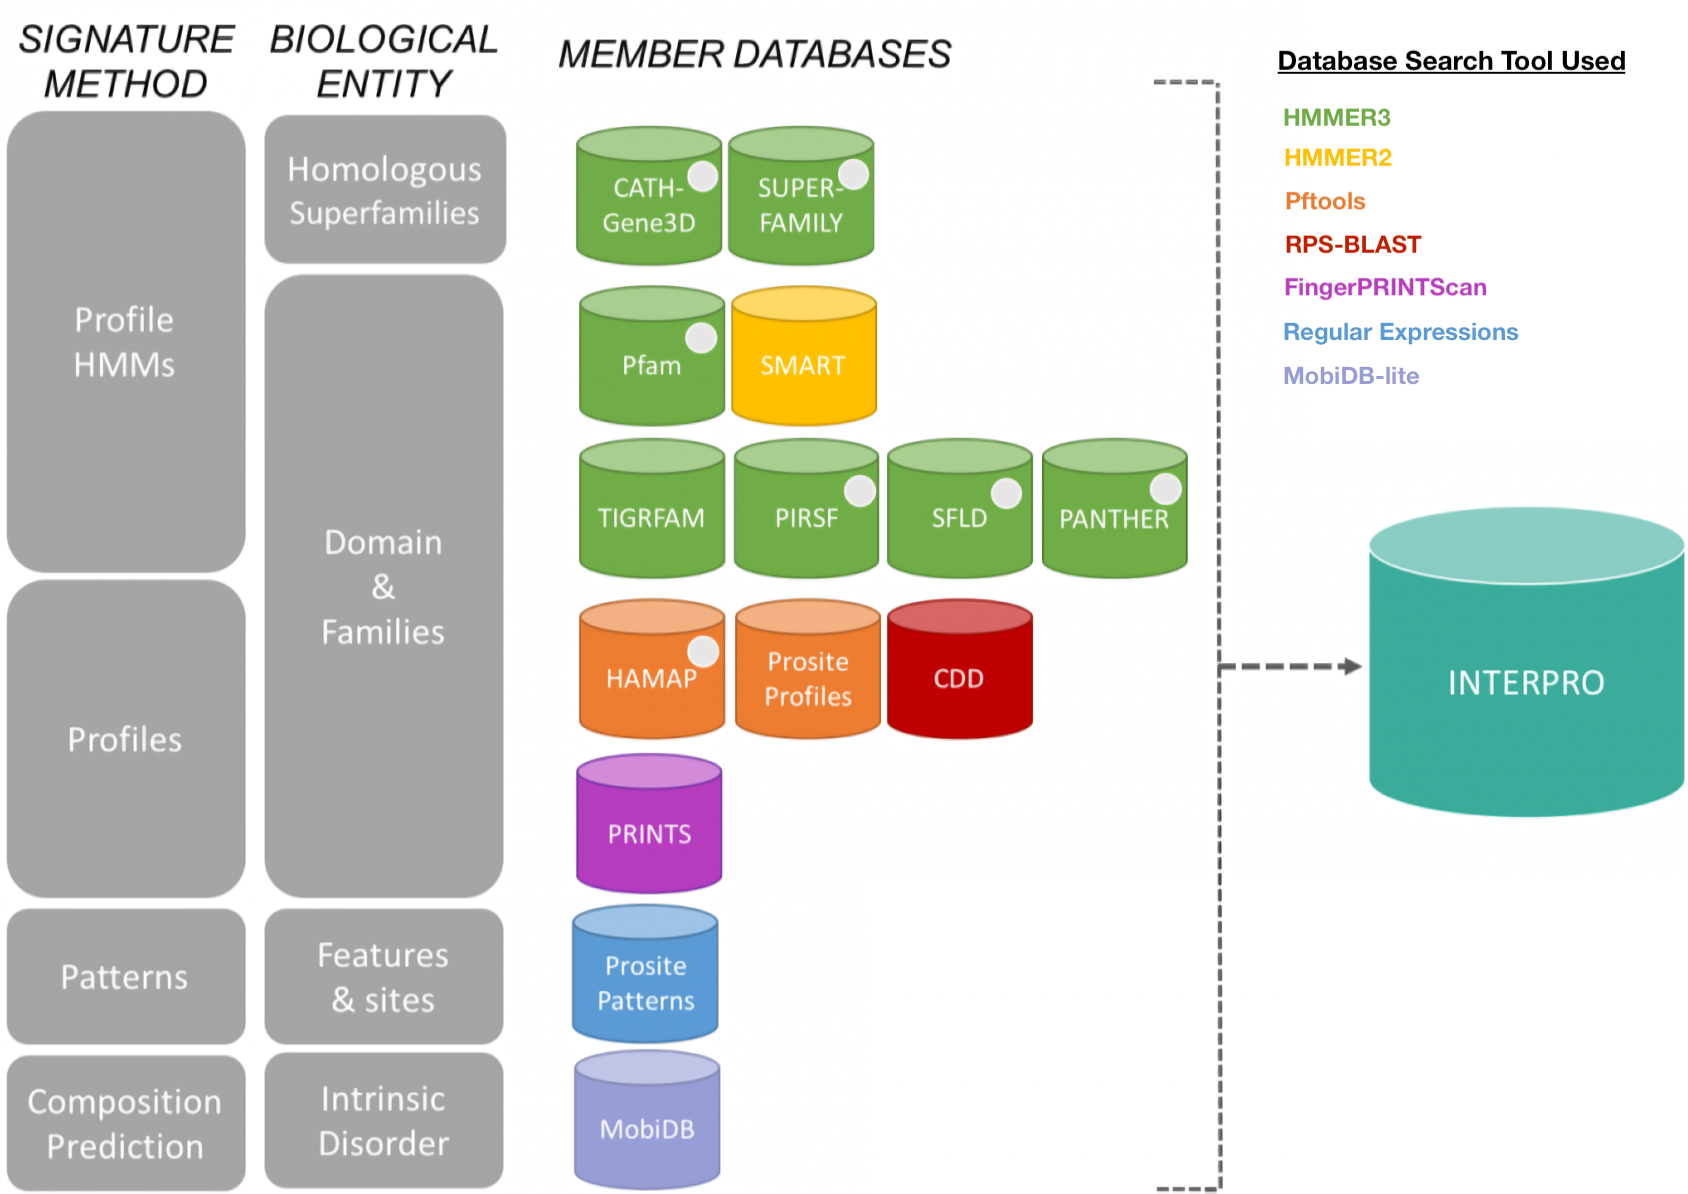
\includegraphics[width=\textwidth]{media/InterPro.png}
	 \caption[The fourteen member databases of the InterPro consortium utilize a 
variety of model-based sequence search techniques to classify novel protein 
sequences.]{\textbf{The fourteen member databases of the InterPro consortium 
utilize a variety of model-based sequence search techniques to classify novel 
protein sequences.} To support these techniques, the databases store models that 
represent multiple proteins or proteins domains. Examples of such models include 
\gls{hmm}s and \gls{pssm}. Examples of software that use such models are HMMER 
\cite{eddy2011accelerated} or \gls{rpsblast} \cite{mcginnis2004blast}. This figure is 
modified from the one found at 
\href{https://www.ebi.ac.uk/training/online/course/introduction-protein-classification-ebi/protein-classification-resources-ebi-interpro}{https://www.ebi.ac.uk/training/online/course/introduction-protein-classification-ebi/protein-classification-resources-ebi-interpro}.}
	 \label{fig:interpro-databases}
\end{figure}

If a portion of an organism's protein and a model are highly similar in 
sequence, they form a match. The quality of this match can be quantified by 
metrics such as the \gls{eval} score. This \gls{eval} score captures how likely 
it is that the match is a real (\textit{i}.\textit{e}., the organism's protein contains the 
domain) given the chance of finding an equivalent match randomly in other 
proteins. Another metric for match quality is the length of the region of high 
sequence similarity, the alignment, shared between the protein and the database 
domain. If it is determined that a match is of high quality, the aligned region 
of the organism's protein can be assigned the same name and function as the 
domain in the database.  As discussed in Chapter \ref{Pygenprop}, Pygenprop can 
generate Micromeda files that store such match information.

Each member database has algorithms for filtering out false positive matches, 
which are those that occur between a model and a region of a protein that does 
not carry out the same function as the domain that the model represents. The 
member databases perform this filtering by implementing unique cut-off values, 
such as minimum \gls{eval} scores or alignment lengths, that can be used to 
filter out matches that may be spurious. The cut-off values can be made unique 
to each model. 

\section{InterProScan} \label{overview-interproscan}

InterPro consortium created a tool, InterProScan, that allows users to compare a 
novel protein sequence to all domain models found within InterPro member 
databases. InterProScan is a software wrapper for and execution engine of the 
model-based sequence search techniques (\textit{e}.\textit{g}., HMMER \cite{eddy2011accelerated}) 
used by all member databases of the InterPro consortium. It also implements the 
false positive filtering techniques developed for each member database. The 
latest version of the software, InterProScan5, follows a Master/Worker 
architecture (see 
\href{http://en.wikipedia.org/wiki/Master/slave_(technology)}{en.wikipedia.org/wiki/Master/slave\_(technology)}) 
where a master process schedules jobs for many worker processes. Depending on 
the number of \gls{cpu} cores of the computer running InterProScan5, tens to 
hundreds of models can be run against a novel protein simultaneously. Due to its 
architecture, InterProScan5 can also run jobs run across a compute cluster. Due 
to this scalability, InterProScan is capable of domain annotating every protein 
of a microorganism in only a few hours, depending on the computer it is run on 
and the organism's genome size. InterProScan takes a \gls{fasta} file 
\cite{pearson19905} containing an organism's predicted proteins as input and 
writes domain annotations and match data to \gls{tsv} files. The match data 
includes supporting information such as \gls{eval} scores for matches and 
predicted domain start and stop points on the organism's annotated protein.

\section{The Genome Properties Database} \label{genome-properties-overview}

The backbone of Micromeda is the Genome Properties database \cite{Haft2013}. The 
database goes beyond simple metabolism to include other organism capabilities 
such as cell motility (\textit{e}.\textit{g}., the presence flagella) and even microbial viral 
immunity mechanisms such a CRISPR/Cas9 \cite{horvath2010crispr}. Within the 
database each capability is called a genome property. Multiple steps support 
each property, and each of these is supported by evidence that can be found from 
an organism's genome such as the presence InterPro domains (\textit{e}.\textit{g}., \gls{pfam} 
\cite{bateman2004pfam}, \gls{tigr} \cite{haft2001tigrfams}, or \gls{cdd} 
\cite{marchler2014cdd} domains) in predicted proteins. Several genome properties 
are required as lines of evidence by others, and thus the database forms a 
rooted \gls{dag} (see 
\href{http://en.wikipedia.org/wiki/Directed_acyclic_graph}{en.wikipedia.org/wiki/Directed\_acyclic\_graph}) 
of connected properties. There are five types of genome properties: pathways, 
metapathways, systems, guilds and categories (see 
\href{https://genome-properties.readthedocs.io/en/latest/flatfile.html\#genome-property-types}{https://genome-properties.readthedocs.io/en/latest/flatfile.html\#genome-property-types} 
for details). One of the core goals of the latest release of Genome Properties 
was to expand the database beyond prokaryotic properties to include properties 
that are only possessed by eukaryotes or are shared between prokaryotes and 
eukaryotes. The most recent version of the Genome Properties database has also 
incorporated pathways from MetaCyc \cite{karp2002metacyc}. Section 
\ref{genomeprop-oop} discusses how Pygenprop represents the structure of the 
Genome Properties database in memory.

\subsection{Assignment of Genome Properties to an Organism}

If a specified number of required steps are found within the domain annotations 
of an organism's proteins, then the organism is understood to posses a specific 
genome property. The process of predicting what properties are possessed by an 
organism is called property assignment. To assign properties to an organism, 
InterProScan is first used to domain annotate all of its predicted proteins 
(\textit{e}.\textit{g}., those produced by Prodigal), and these annotations are then combined with 
information from the Genome Properties database to assess what properties are 
supported. Each property in the database is assigned YES, PARTIAL, and NO 
support. With Micromeda, Pygenprop is used to carry out these assessments. The 
Genome Properties database is provided to Pygenprop in the form of a release 
file, whose contents are detailed in the section below. Subsection 
\ref{AssignmentCachingAlgorithm} details the exact algorithms used for 
generating assignments.  

\subsection{Overview of the Genome Properties Flat File Database and Associated 
File Formats} \label{Genome-Properties-Files} 

The Genome Properties database (as of version 2.0) consists of a series of flat 
files that are hosted inside a GitHub repository (see 
\href{http://github.com/ebi-pf-team/genome-properties}{github.com/ebi-pf-team/genome-properties}). 
Information about individual properties is stored in the repository's 
\textbf{data} folder, and within this folder each property is assigned a second 
internal folder containing three files: 

\begin{itemize}
\item A \textbf{DESC} file, that contains information about the property
\item A \textbf{status} file that contains information onto whether the property 
is public or has been manually curated
\item A \textbf{\gls{fasta}} \cite{pearson19905} file containing representative 
protein sequences that carry out the steps a the property
\end{itemize}

The \textbf{data} folder contains information about both public and non-public 
genome properties. 

In addition to the per-property folders, there is also a Genome Properties 
release file located in the \textbf{flatfiles} folder of the repository that 
also contains Genome Properties information. Specifically, this file, called 
\textbf{genomeProperties.txt}, is a concatenation of all the \textbf{DESC} files 
of all public properties. This file is created with each new release of the 
Genome Properties database on GitHub. Below is simplified a folder structure for 
the Genome Properties GitHub repository.

\begin{verbatim}
├── code/ - # The Genome Properties Perl library.
├── data/ - # Data about both public and private properties
│ ├── GenProp0001/
│ │ ├── DESC - # Detailed property information
│ │ ├── FASTA - # Sequences of proteins that carry out steps
│ │ └── status - # Public and manual curation status
│ └── GenProp0002/
│  ├── DESC
│  ├── FASTA
│  └── status
└── flatfiles/
 └── genomeProperties.txt
\end{verbatim}

Pygenprop's Genome Properties database parser (see Section 
\ref{genome-properties-parser}) is capable of parsing both single \textbf{DESC} 
files of individual properties and the concatenated 
\textbf{genomeProperties.txt} release file. The format of \textbf{DESC} files is 
very similar to the Stockholm sequence alignment format used by both the 
\gls{pfam} and \gls{rfam} databases \cite{bateman2004pfam, griffiths2003rfam}. Like 
these file types, \textbf{DESC} files consist of a series of key-value pairs. 
Because these files use different keys than Stockholm, a custom parser had to be 
developed. An example \textbf{DESC} file can be found at 
\href{http://raw.githubusercontent.com/ebi-pf-team/genome-properties/master/data/GenProp0145/DESC}{raw.githubusercontent.com/ebi-pf-team/genome-properties/master/data/GenProp0145/DESC}. 
A table of keys used in  genome properties \textbf{DESC} files can be found at 
\href{https://genome-properties.readthedocs.io/en/latest/flatfile.html#desc-file}{https://genome-properties.readthedocs.io/en/latest/flatfile .html\#desc-file}.

\subsection{Reasoning for the Selection of Genome Properties as Micromeda's 
Pathway Information Source} \label{reason-for-genome-properties-selection}

During the development of Micromeda, there were four reasons for selecting the 
Genome Properties database over other databases and InterProScan over other 
search tools. These reasons are explained below.

One of the primary reasons for using the Genome Properties database and 
InterProScan is that they allow pathway annotations to be built from domains 
identified by model-based search tools such as HMMER \cite{eddy2011accelerated} 
or \gls{rpsblast} \cite{mcginnis2004blast}. When compared to non-position
specific \gls{blast}-based \cite{altschul1990basic} search methods, which are 
commonly used by other pathway annotation systems, these model-based tools are 
better at detecting enzymes whose sequences are phylogenetically divergent from 
those previously known \cite{eddy2011accelerated}. This improved detection 
capability provides Micromeda with an advantage when it is applied to the 
genomes of previously unstudied organisms.

The Genome Properties database being domain-based also provides Micromeda with 
another advantage. It allows Micromeda to detect the presence of enzymes that 
are split across multiple genes or have fused with other proteins. In a recent 
study that focused on confirming genome-predicted amino-acid auxotrophy across a 
variety of bacteria, the authors found that many predicted instances of 
auxotrophy were misannotations \cite{price2018filling}. Many of these 
misannotations were the result of either gene fusions or the enzyme being split 
across multiple genes \cite{price2018filling}. Traditional whole protein 
sequence-based detection methods such as \gls{blast} \cite{altschul1990basic}, 
which are typically used by pathway annotation pipelines based on databases such 
as \gls{kegg}, were shown to miss these enzymes \cite{price2018filling}. For 
example, if previous forms of a protein were all found to be encoded by a single 
gene, such whole sequence methods were shown to filter out versions of the 
enzyme that are split across genes due to inadequate alignment lengths for 
matches to individual subunits \cite{price2018filling}. In contrast, Micromeda 
would determine that the enzymes exist, as InterProScan will detect all required 
domains, whether the proteins are on one gene or multiple.

Another advantage of Genome Properties is that it is freely available under an 
open-source licence and is hosted on GitHub \cite{richardson2018genome}. In 
contrast, two of the most prominent pathway databases, \gls{kegg} and BioCyc 
\cite{karp2005expansion}, have been commercialized. \gls{kegg}'s website is free 
for academic use in terms of using the data held within for hypothesis testing 
(see \href{http://www.kegg.jp/kegg/legal.html}{kegg.jp/kegg/legal.html}). 
However, bulk download of the entire database, as would be required for a 
pathway annotation system such as Micromeda, has a licensing fee of \$2000 
\gls{usd} per year (as of 2019 and see 
\href{https://www.bioinformatics.jp/docs/subscription_fees.pdf}{bioinformatics.jp/docs/subscription\_fees.pdf}). 
This fee increases to \$5000 \gls{usd} per year if a user ``provide[s] any 
outside service using... \gls{kegg} data" (as of 2019 and see 
\href{https://www.bioinformatics.jp/docs/subscription_fees.pdf}{bioinformatics.jp/docs/subscription\_fees.pdf}). 
Thus, if Micromeda were built around the \gls{kegg} database, users creating 
Micromeda files would be required to pay \$2000 \gls{usd} per year, and any user 
hosting Micromeda server, as a public service, would be required to pay \$5000 
\gls{usd} per year. BioCyc follows a similar paid scheme 
(\href{http://metacyc.org/download.shtml}{metacyc.org/download.shtml}). 

The Genome Properties database has also been shown to have comparable coverage, 
in terms of organism proteins used to support the existence of pathways, to 
databases such a \gls{kegg} and Seed Subsystems \cite{richardson2018genome}. 
This coverage was consistent across a variety of microbes from distant taxonomic 
clades \cite{richardson2018genome}. Thus, there is no high-level database 
completeness disadvantage if Micromeda uses the Genome Properties database. 

\section{Summary}

When Micromeda performs pathway annotation, it does so based on the presence of 
InterPro domains found within organisms' predicted proteomes. These domains are 
detected using model-based sequence search software that is orchestrated by 
InterProScan5. The contents of the Genome Properties database is used to map 
from the presence of domains to the presence of genome property steps. The 
presence of steps is used to infer YES, PARTIAL, or NO support for individual 
genome properties. The model-based search techniques used by InterProScan allow 
Micromeda to provide highly accurate and comprehensive results with no licensing 
fees.
